\chapter{Introduction} \label{introduction}

\epigraph{The stars are not lonely, in their shining solitude. They have each other, and they have us.}{Isaac Asimov}

Observations proved that field stars are not always single; many develop in pairs, and many of these binaries are members of triples or higher-order systems. Additionally, the fraction of systems with companions grows with mass (see \cref{fig:stellar_companions}), as a result massive stars are seldomly formed in isolation. In contrast, many intermediate- and high-mass stars are created in binary or higher order multiple systems with $\sim 50\%$ of spectral type B stars be in triples \citep{sana2014southern,moe2017mind}, a percentage which reduces to $\sim 10\%$ for low-mass stars \citep{raghavan2010survey,toonen2014popcorn,moe2017mind}. In these cases, apart from the intrinsic stellar properties, the evolution depends sensitively on the interaction between the system's stellar components. Consequently, triple systems are not as uncommon as we may mistakenly believe, particularly in the concept of high-mass stars.

Although the fundamentals of single and binary evolution have long been acknowledged \citep{postnov2014evolution,toonen2014popcorn}, the long-term evolution of stellar triples remains unknown. In the simple case, stable triple systems, which are hierarchical, namely, consist of an inner and an outer binary orbit, i.e., the tertiary (third object). The secular evolution of such systems is the modification of orbital elements over timescales substantially larger than the system's dynamical timescale. Hence, the presence of the outer star has no influence on the history of the inner binary and the evolution of the inner binary and the tertiary can be discussed independently. In other cases, a third star in orbit around a binary system can drastically influence the system's development
via dynamical interactions, which influence the orbital elements of the inner and outer orbit through changes in energy and angular momentum. Consequently, hierarchical triple star systems can become unstable via triple stellar evolution processes which are unique to systems with multiplicities of higher orders than binaries.
\begin{figure}[H]
    \centering
    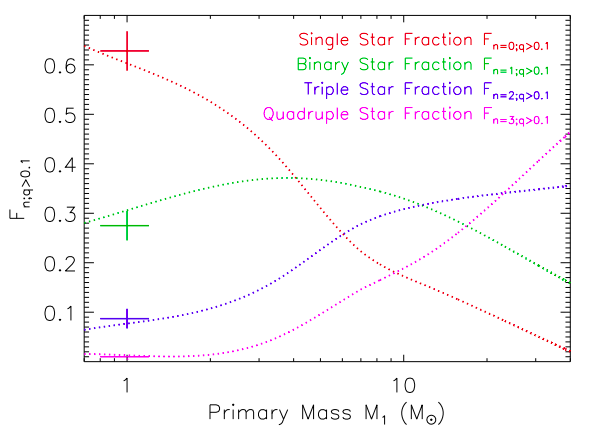
\includegraphics[width=\textwidth]{Thesis/figures/fig_moe_2017.png}
    \caption{Multiplicity fractions as a function of primary mass (dotted lines), including the single-star $F_{n=0;q> 0.1}$ (red), binary-star $F_{n=1;q> 0.1}$ (green), triple-star $F_{n=2;q> 0.1}$ (blue), and quadruple-star fraction $F_{n=3;q> 0.1}$ (magenta). Given a primary mass $M_1$, the model assumes that the multiplicity fractions follow a Poisson distribution across the interval $n = [0, 3]$ in a manner that reproduces the measured multiplicity frequency $F_{mult;q >0.1} = \Sigma_{n=1}^3 \; n F_{n;q> 0.1}$. For solar-type stars, this model matches the measured values (solid) within their uncertainties. Regardless of the uncertainties in the multiplicity fractions, $\leq 10\%$ of O-type stars are single, while $\geq 55\%$ are born in triples and/or quadruples. Figure taken by \cite{moe2017mind}.}
    \label{fig:stellar_companions}
\end{figure}
The rich dynamical behavior of three-body systems can produce Lidov-Kozai cycles, in which the eccentricity of the inner orbit and the inclination between the inner and outer orbits vary periodically \citep{michaely2014secular,toonen2016evolution,mangipudi2022extreme}. As a result, tidal effects (tidal friction), gravitational-wave emission, and stellar interactions such as mass transfer, angular momentum exchange and collisions may be enhanced. In this way, evolution in triples can give rise to stellar mergers \citep{antonini2017binary,silsbee2017lidov,vigna2021massive}, namely some of most energetic events in the universe, ranging from gravitational wave sources to electromagnetic transients, e.g. luminous red novae, and also provide promising evolutionary pathways for exotic objects \citep{sana2012binary, toonen2016evolution}, e.g. blue stragglers \citep{perets2009triple}. In the past, most of our efforts in understanding the progenitors of the events were focused on modeling binary evolution disregarding the interaction of the binary with a third star. Therefore, a detailed examination of triple evolution is as necessary as it is challenging because it demands a self consistent treatment of three-body dynamics and stellar evolution.

\section{Goal \& Scientific Questions}

In this thesis, I investigate a hierarchical triple system in which the tertiary star will eventually overflow its Roche lobe before any of the inner stars leave the main sequence. The goal is to thoroughly examine the mass transfer phase by creating detailed hydrodynamical simulations, evaluate the significance of various parameters in the process, and speculate on the resulting evolution.

There are two main scientific questions that I try to tackle:

\begin{itemize}
    \item How does mass transfer affect the evolution of the inner and outer orbital parameters?
    \item How does the binary's accretion affect the evolution of the inner and outer orbital parameters?
\end{itemize}




\section{Target system: $\xi$ Tau}

$\xi$ Tau is a hierarchical triple system with orbital parameters that are relatively well constrained. The evolution of the system was initially examined by \cite{de2014evolution}, where they  concluded that it is likely to develop \ac{rlof} near the end of the first \ac{agb}, roughly halfway to type B mass transfer \citep{kippenhahn1967entwicklung}.

To further restrict the system's orbital characteristics, \cite{nemravova2016xitauri} combined a large series of spectroscopic photometric (including space-borne) observations with long-baseline optical and infrared spectro-interferometric observations. They show, using perturbation theory, that prominent secular and periodic dynamical effects may be explained by a quadrupole interaction. Despite this, the orbital parameters of the third orbit remain unclear due to the low relative brightness of the most distant star.

I use the orbital parameters given in \cite{2010yCat..73890925T} in my study. The rationale for this is so that I can compare my results to \cite{de2014evolution}. The orbital parameters of $\xi$ Tau are given in \cref{tab:system_orbit_param}.
\begin{table}[H]
    \centering
    \begin{tabular}{|c c c c c c c c|}
       Name & M$_1$ (M$_{\odot}$) & M$_2$ (M$_{\odot}$) &
       M$_3$ (M$_{\odot}$) & $P_{in}$ (day) &
       $P_{out}$ (day) & $\epsilon_{in}$ &
       $\epsilon_{out}$ \\
       \hline
       HD 21364 & 3.2 & 3.1 & 5.5 & 7.15 & 145.5 & 0.0 & 0.15
    \end{tabular}
    \caption{Orbital parameters of $\xi$ Tau system. Masses $M_1$ and $M_2$ correspond to the inner binary components, while $M_3$ is the mass of the tertiary. The orbital period and eccentricity of the inner and outer orbit are given with the subscripts $in$ and $out$, respectively.}
    \label{tab:system_orbit_param}
\end{table}
In their analysis, \cite{nemravova2016xitauri} constrain  the mutual inclination between the two orbits, i.e. the inclination of the outer orbit relative to the inner orbit, concluding that they are nearly coplanar. Mutual inclination, $i_{mut}$, is expected to have the strongest effects on the mass transfer, thus it is a free parameter to be explored.


\section{Thesis outline}

The remainder of this thesis is organized into four chapters. Each chapter starts with a short introduction, while the chapters are structured as follows: 

In the second chapter, I present an overview of single star evolution with a focus on intermediate-mass stars, because this is the mass regime of interest for my target system. I also constrain myself in evolution aspects that are relevant for my hydrodynamical models. Furthermore, I discuss concepts of binary evolution and I argue how to extend these to the triple evolution case. In the remainder of the second chapter, I provide information about the scientific codes, utilized in my simulations. In chapter three, I display the methods used to build my hydrodynamical models, their underlying assumptions and their physical justification. Furthermore, I present the initial setup of my simulations. In chapter four, I demonstrate my results, while a detailed discussion follows in chapter five.






